% Options for packages loaded elsewhere
\PassOptionsToPackage{unicode}{hyperref}
\PassOptionsToPackage{hyphens}{url}
\PassOptionsToPackage{dvipsnames,svgnames*,x11names*}{xcolor}
%
\documentclass[
  english,
  man,floatsintext]{apa6}
\usepackage{amsmath,amssymb}
\usepackage{lmodern}
\usepackage{ifxetex,ifluatex}
\ifnum 0\ifxetex 1\fi\ifluatex 1\fi=0 % if pdftex
  \usepackage[T1]{fontenc}
  \usepackage[utf8]{inputenc}
  \usepackage{textcomp} % provide euro and other symbols
\else % if luatex or xetex
  \usepackage{unicode-math}
  \defaultfontfeatures{Scale=MatchLowercase}
  \defaultfontfeatures[\rmfamily]{Ligatures=TeX,Scale=1}
\fi
% Use upquote if available, for straight quotes in verbatim environments
\IfFileExists{upquote.sty}{\usepackage{upquote}}{}
\IfFileExists{microtype.sty}{% use microtype if available
  \usepackage[]{microtype}
  \UseMicrotypeSet[protrusion]{basicmath} % disable protrusion for tt fonts
}{}
\makeatletter
\@ifundefined{KOMAClassName}{% if non-KOMA class
  \IfFileExists{parskip.sty}{%
    \usepackage{parskip}
  }{% else
    \setlength{\parindent}{0pt}
    \setlength{\parskip}{6pt plus 2pt minus 1pt}}
}{% if KOMA class
  \KOMAoptions{parskip=half}}
\makeatother
\usepackage{xcolor}
\IfFileExists{xurl.sty}{\usepackage{xurl}}{} % add URL line breaks if available
\IfFileExists{bookmark.sty}{\usepackage{bookmark}}{\usepackage{hyperref}}
\hypersetup{
  pdftitle={Morphological and Frequency Effects in Heritage Spanish and the Preterit with States},
  pdfauthor={Patrick D. Thane1},
  pdflang={en-EN},
  pdfkeywords={\texttt{papaja}, heritage languages, preterit-imperfect, Spanish bilingualism},
  colorlinks=true,
  linkcolor=blue,
  filecolor=Maroon,
  citecolor=Blue,
  urlcolor=Blue,
  pdfcreator={LaTeX via pandoc}}
\urlstyle{same} % disable monospaced font for URLs
\usepackage{graphicx}
\makeatletter
\def\maxwidth{\ifdim\Gin@nat@width>\linewidth\linewidth\else\Gin@nat@width\fi}
\def\maxheight{\ifdim\Gin@nat@height>\textheight\textheight\else\Gin@nat@height\fi}
\makeatother
% Scale images if necessary, so that they will not overflow the page
% margins by default, and it is still possible to overwrite the defaults
% using explicit options in \includegraphics[width, height, ...]{}
\setkeys{Gin}{width=\maxwidth,height=\maxheight,keepaspectratio}
% Set default figure placement to htbp
\makeatletter
\def\fps@figure{htbp}
\makeatother
\setlength{\emergencystretch}{3em} % prevent overfull lines
\providecommand{\tightlist}{%
  \setlength{\itemsep}{0pt}\setlength{\parskip}{0pt}}
\setcounter{secnumdepth}{-\maxdimen} % remove section numbering
% Make \paragraph and \subparagraph free-standing
\ifx\paragraph\undefined\else
  \let\oldparagraph\paragraph
  \renewcommand{\paragraph}[1]{\oldparagraph{#1}\mbox{}}
\fi
\ifx\subparagraph\undefined\else
  \let\oldsubparagraph\subparagraph
  \renewcommand{\subparagraph}[1]{\oldsubparagraph{#1}\mbox{}}
\fi
% Manuscript styling
\usepackage{upgreek}
\captionsetup{font=singlespacing,justification=justified}

% Table formatting
\usepackage{longtable}
\usepackage{lscape}
% \usepackage[counterclockwise]{rotating}   % Landscape page setup for large tables
\usepackage{multirow}		% Table styling
\usepackage{tabularx}		% Control Column width
\usepackage[flushleft]{threeparttable}	% Allows for three part tables with a specified notes section
\usepackage{threeparttablex}            % Lets threeparttable work with longtable

% Create new environments so endfloat can handle them
% \newenvironment{ltable}
%   {\begin{landscape}\begin{center}\begin{threeparttable}}
%   {\end{threeparttable}\end{center}\end{landscape}}
\newenvironment{lltable}{\begin{landscape}\begin{center}\begin{ThreePartTable}}{\end{ThreePartTable}\end{center}\end{landscape}}

% Enables adjusting longtable caption width to table width
% Solution found at http://golatex.de/longtable-mit-caption-so-breit-wie-die-tabelle-t15767.html
\makeatletter
\newcommand\LastLTentrywidth{1em}
\newlength\longtablewidth
\setlength{\longtablewidth}{1in}
\newcommand{\getlongtablewidth}{\begingroup \ifcsname LT@\roman{LT@tables}\endcsname \global\longtablewidth=0pt \renewcommand{\LT@entry}[2]{\global\advance\longtablewidth by ##2\relax\gdef\LastLTentrywidth{##2}}\@nameuse{LT@\roman{LT@tables}} \fi \endgroup}

% \setlength{\parindent}{0.5in}
% \setlength{\parskip}{0pt plus 0pt minus 0pt}

% \usepackage{etoolbox}
\makeatletter
\patchcmd{\HyOrg@maketitle}
  {\section{\normalfont\normalsize\abstractname}}
  {\section*{\normalfont\normalsize\abstractname}}
  {}{\typeout{Failed to patch abstract.}}
\patchcmd{\HyOrg@maketitle}
  {\section{\protect\normalfont{\@title}}}
  {\section*{\protect\normalfont{\@title}}}
  {}{\typeout{Failed to patch title.}}
\makeatother
\shorttitle{Morphological and frequency effects and the preterit}
\keywords{`papaja`, heritage languages, preterit-imperfect, Spanish bilingualism\newline\indent Word count: 2,537}
\usepackage{csquotes}
\ifxetex
  % Load polyglossia as late as possible: uses bidi with RTL langages (e.g. Hebrew, Arabic)
  \usepackage{polyglossia}
  \setmainlanguage[]{english}
\else
  \usepackage[main=english]{babel}
% get rid of language-specific shorthands (see #6817):
\let\LanguageShortHands\languageshorthands
\def\languageshorthands#1{}
\fi
\ifluatex
  \usepackage{selnolig}  % disable illegal ligatures
\fi
\newlength{\cslhangindent}
\setlength{\cslhangindent}{1.5em}
\newlength{\csllabelwidth}
\setlength{\csllabelwidth}{3em}
\newenvironment{CSLReferences}[2] % #1 hanging-ident, #2 entry spacing
 {% don't indent paragraphs
  \setlength{\parindent}{0pt}
  % turn on hanging indent if param 1 is 1
  \ifodd #1 \everypar{\setlength{\hangindent}{\cslhangindent}}\ignorespaces\fi
  % set entry spacing
  \ifnum #2 > 0
  \setlength{\parskip}{#2\baselineskip}
  \fi
 }%
 {}
\usepackage{calc}
\newcommand{\CSLBlock}[1]{#1\hfill\break}
\newcommand{\CSLLeftMargin}[1]{\parbox[t]{\csllabelwidth}{#1}}
\newcommand{\CSLRightInline}[1]{\parbox[t]{\linewidth - \csllabelwidth}{#1}\break}
\newcommand{\CSLIndent}[1]{\hspace{\cslhangindent}#1}

\title{Morphological and Frequency Effects in Heritage Spanish and the Preterit with States}
\author{Patrick D. Thane\textsuperscript{1}}
\date{}


\authornote{

This manuscript has been prepared in fulfillment for the final project for Data Science for Linguists.

The authors made the following contributions. Patrick D. Thane: .

Correspondence concerning this article should be addressed to Patrick D. Thane, Department of Spanish and Portuguese, Rutgers University, Office 5184, 15 Seminary Place, New Brunswick, NJ 07649. E-mail: \href{mailto:pthane@spanport.rutgers.edu}{\nolinkurl{pthane@spanport.rutgers.edu}}

}

\affiliation{\vspace{0.5cm}\textsuperscript{1} Rutgers University}

\abstract{
This manuscript presents the methodology of a project evaluating Spanish heritage bilinguals' (HBs') use of preterit aspect with state verbs. In particular, it addresses how lexical frequency and morphological regularity affect the use of the preterit with state verbs in HBs' productive and receptive tendencies at different proficiency levels. A brief presentation of research questions and hypotheses begins the summary, followed by a review of the experiment and related methodologies. A summary of the statistics follows, and a brief overview of findings concludes this essay. This manuscript has been prepared using \texttt{papaja} and is in fulfillment of the final project for Data Science for Linguists.
}



\begin{document}
\maketitle

\hypertarget{research-questions}{%
\section{Research Questions}\label{research-questions}}

\begin{enumerate}
\def\labelenumi{\arabic{enumi}.}
\tightlist
\item
  Do HB prefer preterit inflections with states in a receptive measure more frequently than in production?
\item
  Does lexical frequency affect HBs' production and selection of preterit morphology with state verbs?
\item
  Do proficiency and morphological regularity modulate the effect of lexical frequency?
\end{enumerate}

\hypertarget{hypotheses}{%
\section{Hypotheses}\label{hypotheses}}

Regarding RQ1, it was predictable that HB would select the preterit with states in a receptive measure more frequently than they would produce this form, owing to asymmetrical productive and receptive capacities that are characteristic of heritage grammars (Perez-Cortes, Putnam, \& Sánchez, 2019). With regards to RQ2, it was likely that lexical frequency would affect HB in both the production task and the receptive measure. Lastly, concerning RQ3, it was plausible that more-proficient HB would be less susceptible to the effects of lexical frequency in both tasks, especially in production. Furthermore, it was plausible that regular verbs would be more susceptible to frequency effects than irregular verbs in both tasks. This finding is attributable to past research that suggests that Spanish speakers store and access irregular verbs as full words, while regular stems are stored separately from their inflections (Bowden, Gelfand, Sanz, \& Ullman, 2010).

\hypertarget{participants}{%
\section{Participants}\label{participants}}

47 HB completed the study, all of whom were living in the northeastern United States at the time of data collection. None of these participants had received immersive bilingual schooling, and had received all of their secondary education in the United States. Participants' parents were from a total of twelve Spanish-speaking countries and territories. Participants reported first exposure to English between birth and age seven.

\hypertarget{materials}{%
\section{Materials}\label{materials}}

\hypertarget{biographical-measures}{%
\subsection{Biographical Measures}\label{biographical-measures}}

The present study contained two biographical measures and two experimental tasks. The first biographical measure was the language experience questionnaire, which solicited each participant's age of acquisition of English and Spanish, national origin, length of residence overseas, and extent of formal instruction in Spanish. In addition, the questionnaire contained ten five-point Likert scales concerning how frequently participants used Spanish across five contexts (at home, at work, in coursework, with friends, and with family members), with one scale for comprehension and a separate scale for production in each context. The final part of the questionnaire contained a frequency and translation measure adapted from Hur, Lopez Otero, and Sanchez (2020). In this section, there was a nine-point Likert scale for each of the lexical items used in the experimental tasks of this study in which participants needed to report the frequency of production of individual words. This procedure verified that the lexical frequencies of verbs from the Davies (2016) corpus aligned with HBs' use of and familiarity with these items. Furthermore, each participant needed to translate each of the verbs used in the experimental tasks to demonstrate familiarity with these items. In addition to the biographical questionnaire, each participant completed a 50-item written Spanish proficiency measure (Montrul \& Slabakova, 2003).

\hypertarget{experimental-tasks}{%
\subsection{Experimental Tasks}\label{experimental-tasks}}

The present study used the Davies (2016) corpus to measure lexical frequency, reporting the lemma frequencies of ten state verbs selected for the experimental tasks. Lemma frequencies encompass the total number of tokens of all derived forms of a particular lexical item, therefore providing a metric of the sum of how frequently all permutations of person, number, tense, aspect, mood, and impersonal forms of a particular verb are used. To maintain morphophonological consistency, all verbs were disyllabic. Five verbs were morphologically regular, while the remaining five were irregular. Both sets of verbs represented a continuum of lexical frequency, such that it was possible to address lexical frequency and morphological regularity distinctly. Table 1 lists these verbs and their lexical frequencies.

\begin{tabular}{l|c|l|c}
\hline
Regulars & Tokens & Irregulars & Tokens.1\\
\hline
amar (to love) & 80,242 & creer (to believe) & 537,246\\
\hline
doler (to hurt) & 69,627 & estar (to be) & 10,180,830\\
\hline
faltar (to lack) & 182,742 & excluir (to exclude) & 53,412\\
\hline
gustar (to please) & 541,858 & haber (there is/there are) & 7,679,109\\
\hline
vivir (to live) & 599,425 & tener (to have) & 8,031,798\\
\hline
\end{tabular}

\textbf{Table 1.} Verbs and their lexical frequencies as reported in Davies (2016).

Because HB often exhibit distinct productive and receptive knowledge of the heritage language (Perez-Cortes, Putnam, \& Sánchez, 2019), the present study incorporated two similarly-structured experimental tasks. Each task contained 50 experimental items, of which 20 pertained to preterit aspect with states and 30 were distractors. The twenty preterit items were organized into four conditions with five stimuli each. Conditions followed a 2 x 2 design based upon morphological regularity and type of adverbial (\emph{durante} and \emph{entre}). Therefore, each of the state verbs in Table 1 appeared once with a prepositional phrase headed by \emph{durante} (for) and once with an prepositional phrase headed by \emph{entre} (between). As De Swart (1998) describes, these prepositions force a perfective interpretation and are expected to ``coerce'' state verbs, which are naturally associated with the imperfect, into the preterit. The 30 items consisted of 25 distractors targeting mood morphology and five fillers expected to elicit imperfect morphology with states. Although the imperfect fillers did not form part of statistical analyses, they acted as verification that participants were able to use both perfective and imperfective morphology in the past. Lack of suppliance of imperfect could signify the loss of the aspectual distinction, such that it would be impossible to discern whether participants were using the preterit as a tense marker for all past forms or as a true marker of perfective aspect.

\hypertarget{elicited-production-task-ept}{%
\subsubsection{Elicited Production Task (EPT)}\label{elicited-production-task-ept}}

The first task was a multimodal elicited production task (EPT), in which participants heard and read a four-sentence description to contextualize each response and needed to complete a sentence fragment using a form of the verb written in parentheses. The first two sentences in the description included bounded events in the preterit, while the third sentence contained a verb carrying imperfect morphology that provided background information. The final sentence provided instructions to the participants. Examples (1) and (2) below were experimental items from the EPT.

\begin{enumerate}
\def\labelenumi{\arabic{enumi}.}
\item
  Daniel llegó a Paris en 2015. Se fue en 2019. Le gustaba mucho vivir allí. Describe su tiempo en París. Durante 4 años\ldots{} {[}vivir{]}.
\item
  A las 2:43 la tierra empezó a temblar. Dejó de sacudir a las 2:48. Paco estaba preocupado por el temblor. Describe la duración del terremoto. Entre las 2:43 y las 2:48\ldots{} {[}haber{]}.
\end{enumerate}

\hypertarget{forced-choice-task-fct}{%
\subsubsection{Forced Choice Task (FCT)}\label{forced-choice-task-fct}}

In the forced choice task (FCT), participants again heard 50 sentences following the same structure as the EPT. Instead of completing the sentence fragment, participants heard and read two single-sentence choices. The two choice sentences were identical with the exception that one option contained a verb with preterit markings, and the other carried imperfect markings. Sentences (3) and (4) are examples from the FCT.

\begin{enumerate}
\def\labelenumi{\arabic{enumi}.}
\setcounter{enumi}{2}
\item
  Renata salió para Londres el domingo pasado. Regresó a Barcelona el sábado. Viajaba mucho para su trabajo. {[}Estuvo/*estaba{]} en Londres durante 6 días.
\item
  Esteban recibió una oferta de trabajo el lunes. Después, rechazó la oferta el viernes. Conseguía muchas ofertas en su juventud. {[}Tuvo/*tenía{]} oferta de trabajo durante 3 días.
\end{enumerate}

\hypertarget{procedure}{%
\section{Procedure}\label{procedure}}

Data collection took place online to accommodate the social distancing guidelines of the coronavirus pandemic concurrent with the present study. Participants signed the IRB consent form and completed the biographical and frequency questionnaire followed by the the DELE proficiency measure independently before data collection, which required approximately 30 minutes in total. Subsequently, the researcher administered the EPT followed by the FCT over Zoom videoconferencing software, which required approximately 45 minutes. The total study duration was approximately 75 minutes. Participants either received course credit or compensation for their participation in the study.

\hypertarget{data-coding-and-variables}{%
\section{Data Coding and Variables}\label{data-coding-and-variables}}

Three generalized linear mixed methods (GLMM) models were carried out to evaluate the research questions. An aggregate model was carried out on data from both tasks, through which it was possible to address the predicted asymmetries between production and interpretation. The second two models evaluated the production and interpretation data, respectively. In each of the models, the criterion was the binary suppliance of the preterit. Production of the preterit resulted in a value of ``1,'' while production of alternative past tense forms received a value of ``0.'' Because it was not possible to determine the impact of lexical frequency on preterit production through the use of modal constructions (that is, whether it was the modal verb or the lexical verb that lead to the use of a particular inflection), periphrastic constructions were eliminated from the data. Furthermore, because it is not possible to distinguish between tense and aspect marking in Spanish nonpast forms, any responses in the present tense were not coded, because the aspectual contrast is exclusive to the past tense and is not represented in the present. Although Cuza, Pérez-Tattam, Barajas, Miller, and Sadowski (2013) report that the present simple is imperfective by definition, and may emerge as an ``avoidance strategy'' for the imperfect, it is not possible to extrapolate whether participants wish to mark tense or aspect when using nonpast forms.

There were four predictors in the present study: task (in the aggregate model only; either EPT or FCT), proficiency (the number of correct responses on the 50-question proficiency measure), lexical frequency (the lemma frequency of each state verb in the Davies (2016) corpus), and morphological regularity (irregular or regular). Therefore, task and regularity formed binary predictors, while proficiency and lexical frequency comprised continuous variables, both of which were standardized prior to analysis. The models also included all two- and three-way interactions between lexical frequency, morphological regularity, and proficiency level. Participant and item were included as random effects.

\hypertarget{descriptive-data}{%
\subsection{Descriptive Data}\label{descriptive-data}}

Figure 1 provides a summary of the average level of use of the preterit with each state verb across participants in both production (EPT) and interpretation (FCT). This summary suggests that with participants' proficiency held constant, it appears (a) that HB were more likely to select the preterit in the FCT than they were to produce this form in the EPT and (b) that production of preterit forms appeared to increase as lexical frequency decreased, which differs from previous findings on lexical frequency (Giancaspro, 2020; Hur, Lopez Otero, \& Sanchez, 2020). Moreover, Figure 2 presents each participant's proportion of preterit use in each task as a function of proficiency. It appeared that proficiency had a more facilitative effect in interpretation of preterit morphology than in production. Taken together, these findings may signal that overall command of Spanish correlates with performance in the receptive FCT, which has lower task demands, while lexical frequency may affect performance due to the difficulty of production.

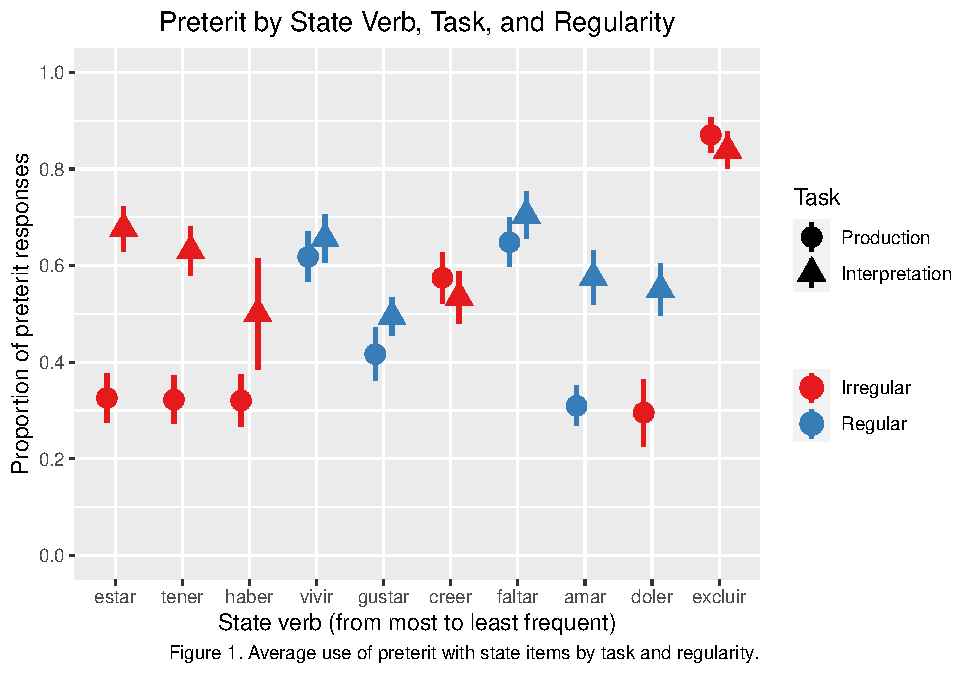
\includegraphics{Final-Manuscript_files/figure-latex/Pret-LI-graph-1.pdf}

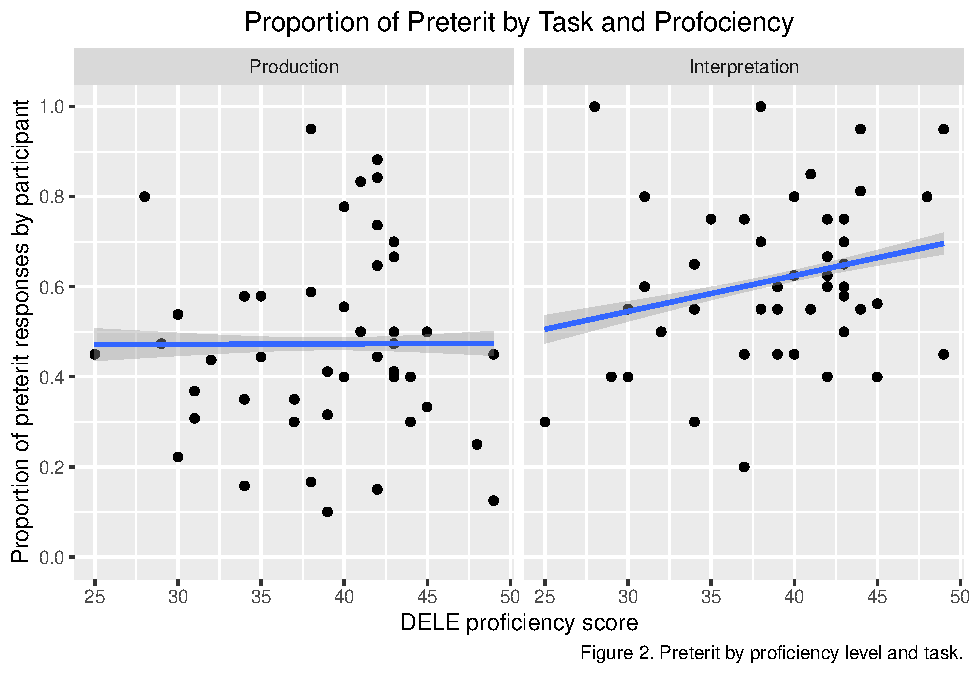
\includegraphics{Final-Manuscript_files/figure-latex/generate-prof-plot-1.pdf}

\hypertarget{statistical-models}{%
\subsection{Statistical Models}\label{statistical-models}}

Results of the three GLMMs carried out in \emph{R} studio for statistical computing are reported below. The Appendix provides statistical figures, and Figures 3 through 5 provide visual summaries of each model.

\hypertarget{aggregate-results}{%
\subsubsection{Aggregate Results}\label{aggregate-results}}

Results in the aggregate model included 1,774 observations. 106 observations (5.6\%) were removed in instances in which participants did not respond to the prompt, did not use a conjugated form of the listed state verb, or produced nonpast forms. Findings revealed a main effect for task (\emph{B} = -0.7464, \emph{p} = .0048) and for lexical frequency (\emph{B} = -0.4925, \emph{p} = .0028), as predicted. However, there were no effects for lexical frequency or morphological regularity at the \emph{p} \textless{} 0.05 level, contra the hypotheses. Figure 2 summarizes the results of the aggregate model.

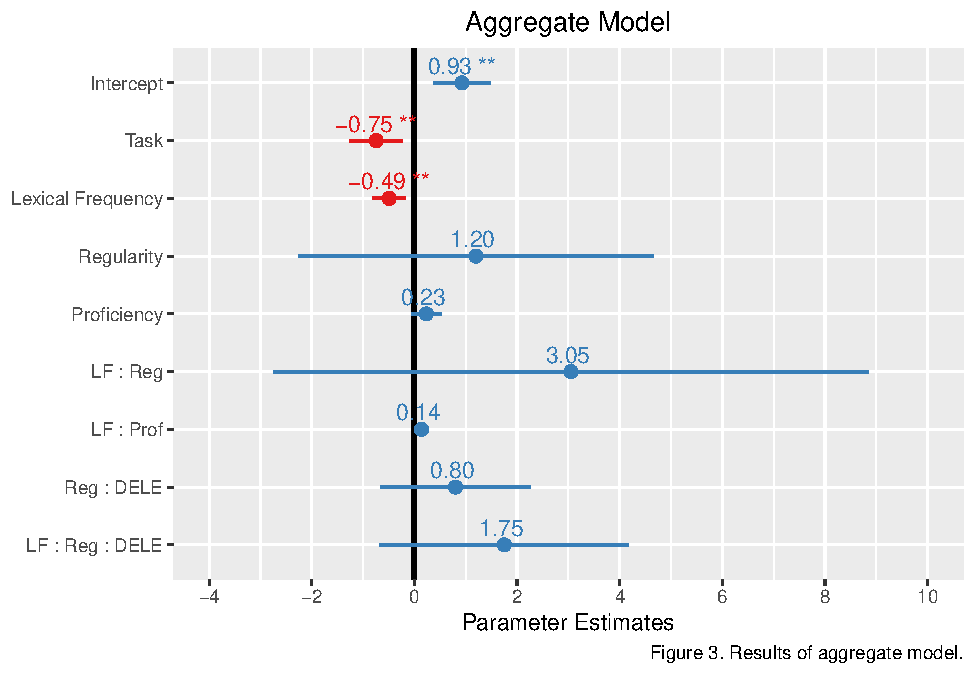
\includegraphics{Final-Manuscript_files/figure-latex/aggregate-model-1.pdf}

\hypertarget{production-results}{%
\subsubsection{Production Results}\label{production-results}}

Results in the EPT included 863 observations. 77 observations (8.1\%) were removed in instances in which participants either substituted a present tense form or used a modal construction. Findings revealed a negative main effect for lexical frequency (\emph{B} = -0.8032, \emph{p} = .0004) and an interaction between proficiency and lexical frequency (\emph{B} = 0.3097, \emph{p} = .0055). There was no effect for the interaction between lexical frequency and morphological regularity at the \emph{p} \textless{} 0.05 level, contra the hypotheses. Note that although the effect for lexical frequency was part of the predictions, the \emph{negative} nature of this correlation suggests a decrease in the productivity of preterit morphology with the most frequent state verbs. Figure 3 summarizes the results of the production model.

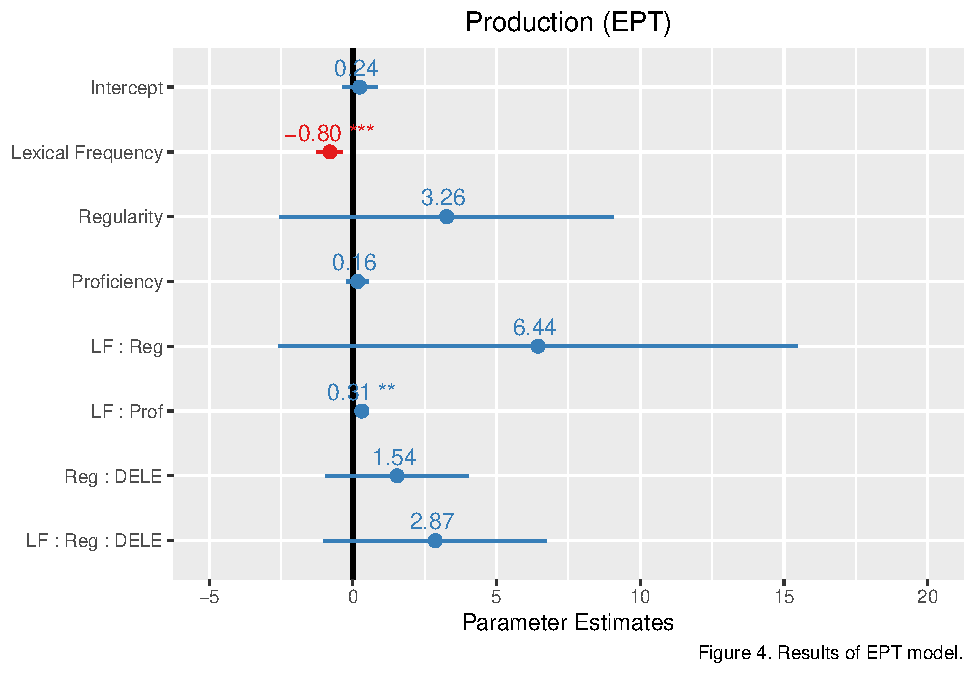
\includegraphics{Final-Manuscript_files/figure-latex/HB-EPT-model-1.pdf}

\hypertarget{fct-results}{%
\subsubsection{FCT Results}\label{fct-results}}

Results in the FCT included 911 observations. 29 observations (3\%) were removed in instances in which participants did not make a selection between either inflection. Findings revealed a main effect for proficiency (\emph{B} = 0.395, \emph{p} = 0.0306); however, there were no effects for lexical frequency or for morphological regularity at the \emph{p} \textless{} 0.05 level, contra the hypotheses. Figure 4 summarizes the results of the FCT.

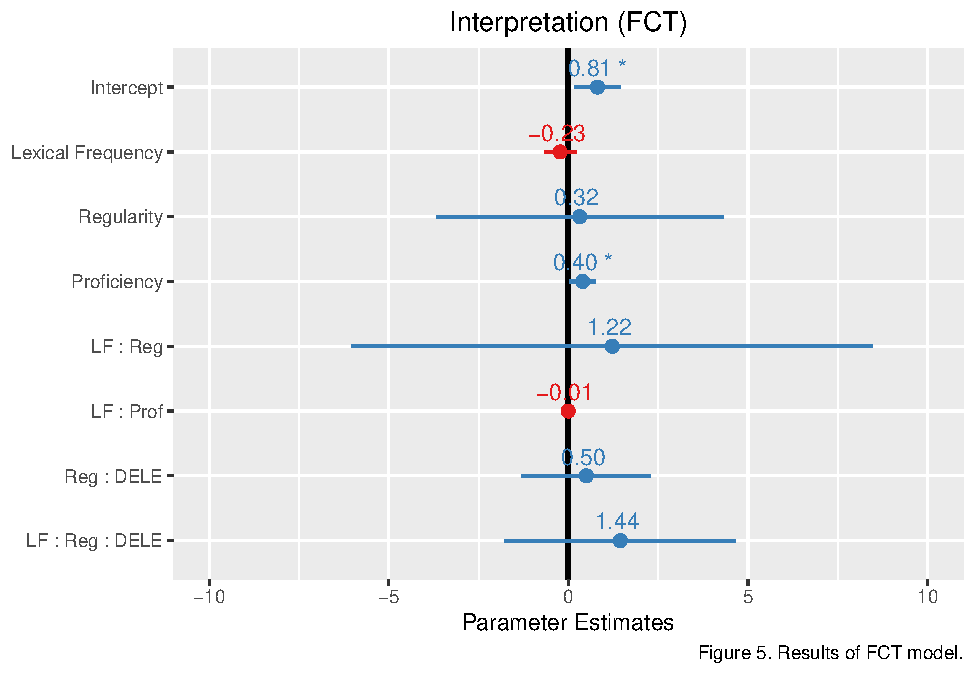
\includegraphics{Final-Manuscript_files/figure-latex/HB-FCT-model-1.pdf}

\hypertarget{nested-model-comparisons-for-production}{%
\subsection{Nested model comparisons for production}\label{nested-model-comparisons-for-production}}

To evaluate the validity of the statistical interaction between proficiency and lexical frequency in production, it was necessary to conduct a nested model comparison of fixed effects in the EPT model. Effects in Table 2 where \emph{p} \textless{} 0.05 accounted for variance in production of the preterit with states. The effect for token frequency, as well as the interaction between proficiency and token frequency, both obtained values where \emph{p} \textless{} 0.05, supporting the findings that more-proficient HB are less susceptible to the impact of lexical frequency in the production of preterit morphology with states, but that less-frequent verbs are more likely to receive preterit inflections in production.

\begin{tabular}{l|c|c|c|c|c|c|c}
\hline
Model & Akaike & Bayesian & Likelihood & Deviance & Chisquare & DF & p\\
\hline
Intercept & 1052.777 & 1067.058 & -523.3883 & 1046.777 & NA & NA & NA\\
\hline
Frequency & 1049.419 & 1068.461 & -520.7097 & 1041.419 & 5.3572857 & 1 & 0.0206359\\
\hline
Regularity & 1048.515 & 1072.317 & -519.2574 & 1038.515 & 2.9046074 & 1 & 0.0883268\\
\hline
Proficiency & 1050.515 & 1079.077 & -519.2574 & 1038.515 & 0.0000022 & 1 & 0.9988275\\
\hline
Freq:Reg & 1050.762 & 1084.084 & -518.3808 & 1036.762 & 1.7531364 & 1 & 0.1854829\\
\hline
Freq:Prof & 1032.200 & 1070.284 & -508.1002 & 1016.200 & 20.5611652 & 1 & 0.0000058\\
\hline
\end{tabular}

\hypertarget{summary}{%
\subsection{Summary}\label{summary}}

The results suggest that in production, preterit use is correlated with \emph{less} frequent verbs. Such findings point to morphological defaults, which is consistent with previous literature (e.g, Silva-Corvalan (1994) for longitudinal data on the simplification of verbal morphology in Spanish HB). English lacks an aspectual contrast; therefore, following Giorgi and Pianesi (1997)'s analysis, English instantiates the {[}+perfective{]} feature that is associated with the Spanish preterit, but does not mark {[}-perfective{]} forms distinctly. As a result, the preterit can be interpreted as the ``unmarked'' form (McCarthy, 2004), and may act as a default marker for all past tense forms either when it is too cognitively taxing to retrieve the imperfect under performative pressures or as a result of the restructuring of the aspect system in bilingual grammars at the representational level. However, the use of states is strongly associated with imperfect morphology, even where the preterit would be preferred with eventive predicates (Cuza, Pérez-Tattam, Barajas, Miller, \& Sadowski, 2013; Montrul, 2002; Potowski, 2005; Silva-Corvalan, 1994), including in monolingual varieties (Wulff, Ellis, Römer, Bardovi-Harlig, \& Leblanc, 2009). Therefore, the use of perfective aspect may surface as a default or ``elsewhere form'' in infrequently-used states under the pressures of production, while the imperfect-state relationship remains in place at high levels of lexical frequency. Only those HB who have higher proficiency in Spanish appear to be able to ``override'' the defaults for preterit and imperfective morphology respectively, attending instead to the coercive nature of the adverbials \emph{durante} and \emph{entre}, which signal a perfective interpretation. Despite the interrelatedness of proficiency and lexical frequency as predictors of defaults in production, there was no role for morphological regularity in the present study.

In contrast, receptive data from the FCT suggest that proficiency is the lone predictor for the use of preterit morphology with states, and that neither morphological regularity nor lexical frequency appeared to affect HB in their selectional preferences for aspect with state verbs. Proficiency and receptive tasks such as the FCT in the present study are thought to reflect speakers' competence, mitigating performance pressures that can surface in production (Perez-Cortes, Putnam, \& Sánchez, 2019). Therefore, frequency may modulate the selection of morphological defaults due to performative challenges during production, while proficiency accounts for variability at the representational level. Consequently, the correlation between use of the preterit and proficiency in the interpretative domain is more reflective of speakers' knowledge of aspect morphology, while lexical frequency can be interpreted as evidence of performative difficulties in production.

\begin{center}\rule{0.5\linewidth}{0.5pt}\end{center}

\hypertarget{appendix-statistical-results}{%
\section{Appendix: Statistical Results}\label{appendix-statistical-results}}

\begin{table}

\caption{\label{tab:table-for-aggregate}Table 3. Results of GLMM for aggregate model.}
\centering
\begin{tabular}[t]{l|c|c|c|c|c|c}
\hline
Predictor & Estimate & SE & z & p & CILower & CIUpper\\
\hline
(Intercept) & 0.9250791 & 0.2841020 & 3.2561511 & 0.0011293 & 0.3682494 & 1.4819088\\
\hline
Task (EPT) & -0.7463962 & 0.2646805 & -2.8199891 & 0.0048025 & -1.2651604 & -0.2276319\\
\hline
Frequency & -0.4925115 & 0.1652754 & -2.9799453 & 0.0028830 & -0.8164453 & -0.1685778\\
\hline
Regularity & 1.1980114 & 1.7615853 & 0.6800757 & 0.4964565 & -2.2546324 & 4.6506552\\
\hline
Proficiency & 0.2316422 & 0.1499923 & 1.5443599 & 0.1225012 & -0.0623374 & 0.5256217\\
\hline
Frequency:Regularity & 3.0498723 & 2.9592972 & 1.0306069 & 0.3027252 & -2.7502437 & 8.8499883\\
\hline
Frequency:Proficiency & 0.1369687 & 0.0722178 & 1.8966057 & 0.0578800 & -0.0045756 & 0.2785130\\
\hline
Regularity:Proficiency & 0.7992227 & 0.7430601 & 1.0755828 & 0.2821139 & -0.6571483 & 2.2555936\\
\hline
3-Way Interation & 1.7503203 & 1.2369708 & 1.4150054 & 0.1570669 & -0.6740979 & 4.1747386\\
\hline
\end{tabular}
\end{table}

\begin{table}

\caption{\label{tab:create-EPT-table}Table 4. Results of GLMM for EPT.}
\centering
\begin{tabular}[t]{l|c|c|c|c|c|c}
\hline
Predictor & Estimate & SE & z & p & CILower & CIUpper\\
\hline
(Intercept) & 0.2369789 & 0.3139082 & 0.7549307 & 0.4502906 & -0.3782698 & 0.8522277\\
\hline
Frequency & -0.8032309 & 0.2288721 & -3.5095181 & 0.0004489 & -1.2518121 & -0.3546498\\
\hline
Regularity & 3.2625644 & 2.9613242 & 1.1017248 & 0.2705813 & -2.5415245 & 9.0666533\\
\hline
Proficiency & 0.1643294 & 0.1966037 & 0.8358406 & 0.4032446 & -0.2210069 & 0.5496657\\
\hline
Frequency:Regularity & 6.4439345 & 4.6065067 & 1.3988766 & 0.1618500 & -2.5846527 & 15.4725218\\
\hline
Frequency:Proficiency & 0.3097190 & 0.1116582 & 2.7738141 & 0.0055403 & 0.0908730 & 0.5285650\\
\hline
Regularity:Proficiency & 1.5446856 & 1.2666181 & 1.2195354 & 0.2226410 & -0.9378402 & 4.0272114\\
\hline
3-Way Interation & 2.8651491 & 1.9809823 & 1.4463274 & 0.1480854 & -1.0175049 & 6.7478031\\
\hline
\end{tabular}
\end{table}

\begin{table}

\caption{\label{tab:create-FCT-table}Table 5. Results of GLMM for FCT.}
\centering
\begin{tabular}[t]{l|c|c|c|c|c|c}
\hline
Predictor & Estimate & SE & z & p & CILower & CIUpper\\
\hline
(Intercept) & 0.8083824 & 0.3328710 & 2.4285154 & 0.0151608 & 0.1559672 & 1.4607975\\
\hline
Frequency & -0.2266094 & 0.2298915 & -0.9857232 & 0.3242690 & -0.6771886 & 0.2239697\\
\hline
Regularity & 0.3157047 & 2.0404348 & 0.1547242 & 0.8770387 & -3.6834741 & 4.3148835\\
\hline
Proficiency & 0.3950016 & 0.1826508 & 2.1626048 & 0.0305716 & 0.0370125 & 0.7529907\\
\hline
Frequency:Regularity & 1.2216921 & 3.7001890 & 0.3301702 & 0.7412714 & -6.0305451 & 8.4739292\\
\hline
Frequency:Proficiency & -0.0068696 & 0.1014293 & -0.0677277 & 0.9460024 & -0.2056673 & 0.1919281\\
\hline
Regularity:Proficiency & 0.4987351 & 0.9168866 & 0.5439441 & 0.5864800 & -1.2983297 & 2.2957998\\
\hline
3-Way Interation & 1.4423997 & 1.6393029 & 0.8798860 & 0.3789211 & -1.7705750 & 4.6553743\\
\hline
\end{tabular}
\end{table}

\begin{center}\rule{0.5\linewidth}{0.5pt}\end{center}

\hypertarget{references}{%
\section{References}\label{references}}

\setlength{\parindent}{-0.5in}
\setlength{\leftskip}{0.5in}

\hypertarget{refs}{}
\begin{CSLReferences}{1}{0}
\leavevmode\hypertarget{ref-bowden_verbal_2010}{}%
Bowden, H. W., Gelfand, M. P., Sanz, C., \& Ullman, M. T. (2010). Verbal {Inflectional} {Morphology} in {L1} and {L2} {Spanish}: {A} {Frequency} {Effects} {Study} {Examining} {Storage} {Versus} {Composition}. \emph{Language Learning}, \emph{60}(1), 44--87. \url{https://doi.org/10.1111/j.1467-9922.2009.00551.x}

\leavevmode\hypertarget{ref-schwieter_chapter_2013}{}%
Cuza, A., Pérez-Tattam, R., Barajas, E., Miller, L., \& Sadowski, C. (2013). Chapter 9. {The} development of tense and aspect morphology in child and adult heritage speakers. In J. W. Schwieter (Ed.), \emph{Language {Learning} \& {Language} {Teaching}} (Vol. 38, pp. 193--220). Amsterdam: John Benjamins Publishing Company. \url{https://doi.org/10.1075/lllt.38.12cuz}

\leavevmode\hypertarget{ref-davies_corpus_2016}{}%
Davies, M. (2016). \emph{Corpus del {Español}: {Two} billion words, 21 countries. {Available} online at http://www.corpusdelespanol.org/web-dial/. ({Web} / {Dialects})}.

\leavevmode\hypertarget{ref-de_swart_aspect_1998}{}%
De Swart, H. (1998). Aspect shift and coercion. \emph{Natural Language and Linguistic Theory}, \emph{16}(2), 347--385. \url{https://doi.org/10.1023/A:1005916004600}

\leavevmode\hypertarget{ref-brehmer_not_2020}{}%
Giancaspro, D. (2020). Not in the mood: {Frequency} effects in heritage speakers' subjunctive knowledge. In B. Brehmer \& J. Treffers-Daller (Eds.), \emph{Studies in {Bilingualism}} (Vol. 59, pp. 72--97). Amsterdam: John Benjamins Publishing Company. \url{https://doi.org/10.1075/sibil.59.03gia}

\leavevmode\hypertarget{ref-giorgi_tense_1997}{}%
Giorgi, A., \& Pianesi, F. (1997). \emph{Tense and aspect: From semantics to morphosyntax}. New York: Oxford University Press.

\leavevmode\hypertarget{ref-hur_gender_2020}{}%
Hur, E., Lopez Otero, J. C., \& Sanchez, L. (2020). Gender {Agreement} and {Assignment} in {Spanish} {Heritage} {Speakers}: {Does} {Frequency} {Matter}? \emph{Languages}, \emph{5}(4), 48. \url{https://doi.org/10.3390/languages5040048}

\leavevmode\hypertarget{ref-mccarthy_underspecification_2004}{}%
McCarthy, C. (2004). Underspecification and {Default} {Morphology} in {Second} {Language} {Spanish}, 12.

\leavevmode\hypertarget{ref-montrul_incomplete_2002}{}%
Montrul, S. (2002). Incomplete acquisition and attrition of {Spanish} tense/aspect distinctions in adult bilinguals. \emph{Bilingualism: Language and Cognition}, \emph{5}(01). \url{https://doi.org/10.1017/S1366728902000135}

\leavevmode\hypertarget{ref-montrul_competence_2003}{}%
Montrul, S., \& Slabakova, R. (2003). {COMPETENCE} {SIMILARITIES} {BETWEEN} {NATIVE} {AND} {NEAR}-{NATIVE} {SPEAKERS}: {An} {Investigation} of the {Preterite}-{Imperfect} {Contrast} in {Spanish}. \emph{Studies in Second Language Acquisition}, \emph{25}(3), 351--398. \url{https://doi.org/10.1017/S0272263103000159}

\leavevmode\hypertarget{ref-perez-cortes_differential_2019}{}%
Perez-Cortes, Putnam, \& Sánchez. (2019). Differential {Access}: {Asymmetries} in {Accessing} {Features} and {Building} {Representations} in {Heritage} {Language} {Grammars}. \emph{Languages}, \emph{4}(4), 81. \url{https://doi.org/10.3390/languages4040081}

\leavevmode\hypertarget{ref-potowski_tense_2005}{}%
Potowski, K. (2005). Tense and {Aspect} in the {Oral} and {Written} {Narratives} of {Two}-{Way} {Immersion} {Students}, 15.

\leavevmode\hypertarget{ref-silva-corvalan_language_1994}{}%
Silva-Corvalan, C. (1994). \emph{Language contact and change: {Spanish} in {Los} {Angeles}}. Oxford : New York: Clarendon Press ; Oxford University Press.

\leavevmode\hypertarget{ref-wulff_acquisition_2009}{}%
Wulff, S., Ellis, N. C., Römer, U., Bardovi-Harlig, K., \& Leblanc, C. J. (2009). The {Acquisition} of {Tense}-{Aspect}: {Converging} {Evidence} {From} {Corpora} and {Telicity} {Ratings}. \emph{The Modern Language Journal}, \emph{93}(3), 354--369. \url{https://doi.org/10.1111/j.1540-4781.2009.00895.x}

\end{CSLReferences}


\end{document}
